\chapter{Reinforcement Learning Foundations}
\label{chap:rl_basis}

Reinforcement learning is the branch of machine learning concerned with sequential decision-making. Historically, RL emerged from the confluence of two research threads~\cite{suttonReinforcementLearningIntroduction2020}: \emph{trial-and-error learning}, in which actions followed by favorable outcomes are reinforced; and \emph{dynamic programming}, which solves sequential decision problems through value functions and the Bellman equations~\cite{bellmanDynamicProgramming1957}. Modern RL combines both: an agent learns directly from interaction with an environment, guided by value functions, to maximize a cumulative reward signal. As illustrated in Figure~\ref{fig:RL-MDP}, at each step $t$ the agent observes state $S_t$ and reward $R_t$ from the previous transition, selects action $A_t$, and the environment transitions to $S_{t+1}$, returning $R_{t+1}$. Throughout this chapter, capital letters $S_t, A_t, R_t$ denote random variables and lowercase $s, a, r$ their realizations\footnote{Inside expectations, lowercase symbols are used as dummy integration variables, following standard convention in the RL literature.}.

\begin{figure}[!htb]
  \centering
  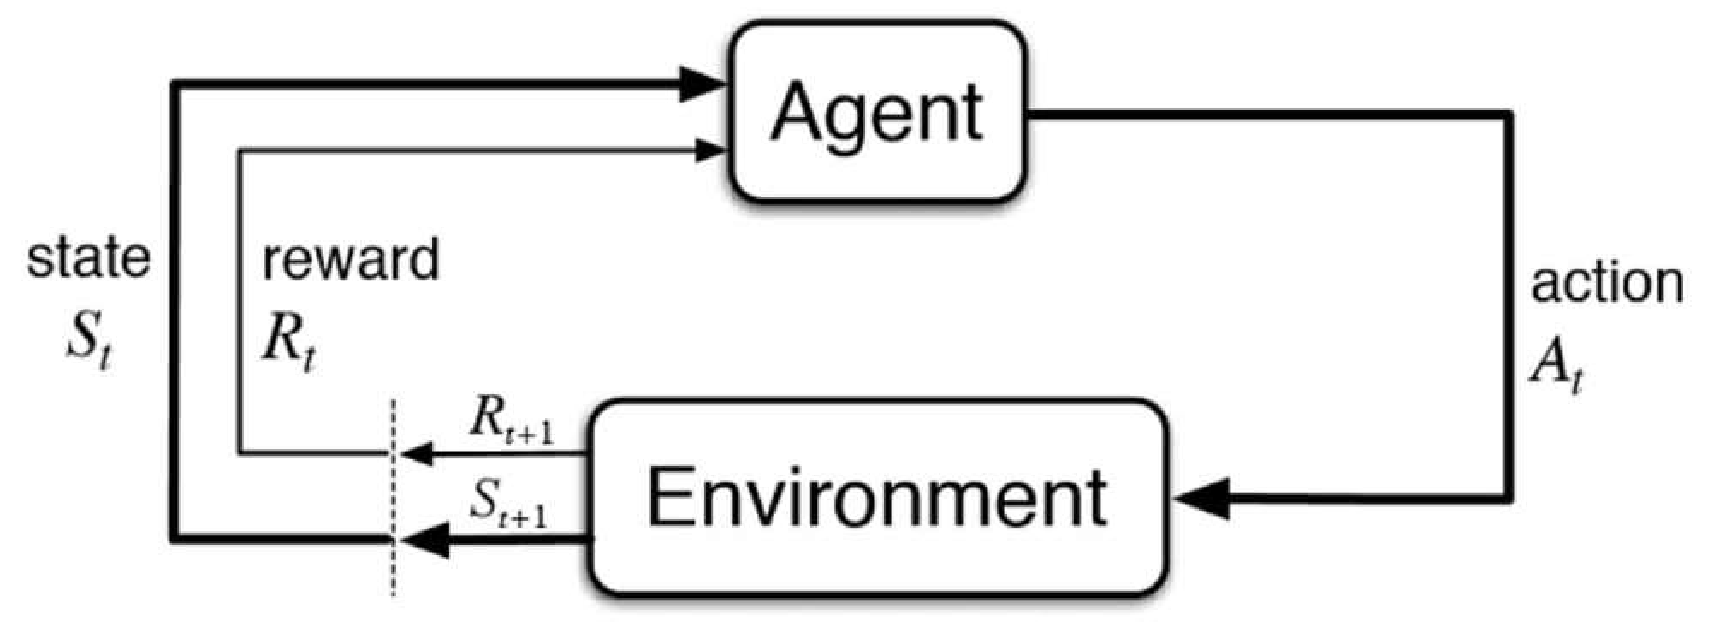
\includegraphics[width=\textwidth]{chapters/03_reinforcement_learning/figures/RL-MDP.pdf}
  \caption[Agent-environment interaction loop (MDP)]{The agent-environment interaction loop in a Markov Decision Process~\cite{suttonReinforcementLearningIntroduction2020}.}
  \label{fig:RL-MDP}
\end{figure}

This chapter introduces the core RL concepts used throughout this thesis, building on the MDP notation in Chapter~\ref{chap:background}. 
It progresses from value functions and policies to policy-gradient methods and PPO, the algorithm underlying all RL agents in this thesis. Section~\ref{sec:ppo-overview} concludes with a visual overview of the full PPO training loop instantiated for MicroRTS.

\section{Policies and Value Functions}

In RL, an agent selects actions according to a \emph{policy} $\pi(a \mid s) = \mathbb{P}(A_t = a \mid S_t = s)$, which may be deterministic or stochastic. The outcome from timestep $t$ is captured by the \emph{discounted return}:
\begin{align}
G_t = \sum_{k=0}^{T-t-1} \gamma^k R_{t+k+1}.
\label{eq:G_t}
\end{align}
To quantify the quality of a policy, two \emph{value functions} are defined. The \emph{state-value function} measures the expected discounted return when starting from state $s$ and following $\pi$:
\begin{align}
V^\pi(s) = \mathbb{E}_\pi\!\left[ G_t \mid S_t = s \right],
\end{align}

while the \emph{action-value function} additionally conditions on the first action taken:
\begin{align}
Q^\pi(s,a) = \mathbb{E}_\pi\!\left[ G_t \mid S_t = s,\; A_t = a \right].
\end{align}
Both satisfy the \emph{Bellman expectation equations}~\cite{bellmanDynamicProgramming1957}, which follow from the recursive structure of $G_t$:
\begin{align}
V^\pi(s) = \sum_{a \in \mathcal{A}} \pi(a \mid s) \sum_{s' \in \mathcal{S}} \mathcal{T}(s, a, s') \left[ \mathcal{R}(s, a, s') + \gamma V^\pi(s') \right], \label{eq:bellman_v} \\[6pt]
Q^\pi(s,a) = \sum_{s' \in \mathcal{S}} \mathcal{T}(s, a, s') \left[ \mathcal{R}(s, a, s') + \gamma \sum_{a' \in \mathcal{A}} \pi(a' \mid s')\, Q^\pi(s', a') \right]. \label{eq:bellman_q}
\end{align}
% V^\pi(s) &= \sum_{a \in \mathcal{A}} \pi(a \mid s) \left[ \mathcal{R}(s, a) + \gamma \sum_{s' \in \mathcal{S}} \mathcal{T}(s, a, s')\, V^\pi(s') \right], \label{eq:bellman_v} \\[6pt]
% Q^\pi(s,a) &= \mathcal{R}(s,a) + \gamma \sum_{s' \in \mathcal{S}} \mathcal{T}(s, a, s') \sum_{a' \in \mathcal{A}} \pi(a' \mid s')\, Q^\pi(s', a'). \label{eq:bellman_q}

The \emph{optimal policy} $\pi^*$ is the one that achieves the highest state-value in every state simultaneously:
\begin{align}
V^{\pi^*}(s) \geq V^\pi(s), \quad \forall \pi, \; \forall s \in \mathcal{S}.
\end{align}
Bellman's optimality theorem~\cite{bellmanDynamicProgramming1957} guarantees the existence of such a policy in finite MDPs.

\section{Core RL Paradigms}

\subsection{Model-Free vs Model-Based}

Model-free methods learn a policy or value function directly from interaction with the environment, treating it as a black box. Model-based methods instead build or use an explicit model of the transition dynamics $\mathcal{T}(s,a,s')$ and reward function $\mathcal{R}(s,a,s')$, which they use to plan ahead. While more sample-efficient in principle, model-based approaches require an accurate model of the environment: a condition difficult to meet in RTS games, where the action space is combinatorially large and transitions depend on the opponent's unknown actions. Model-free methods, especially policy-gradient methods, are therefore common in modern DRL approaches to RTS games.

\subsection{On-Policy vs Off-Policy}

On-policy methods optimize the policy using data collected by the current policy itself; after each update, previous data becomes stale. Off-policy methods can reuse data from past policies through experience replay buffers, improving sample efficiency at the cost of distribution mismatch between the \emph{behavior policy} (which generated the data) and 
the \emph{target policy} (being optimized)~\cite{suttonReinforcementLearningIntroduction2020}. In RTS settings, on-policy methods are typically preferred in practice: the non-stationarity introduced by opponent adaptation and curriculum learning causes replay data to become rapidly outdated, undermining the key advantage of off-policy approaches. AlphaStar~\cite{vinyalsGrandmasterLevelStarCraft2019} stands as a notable exception, discussed in detail in Section~\ref{sec:alphastar}.

\section{Value-Based vs Policy-Based Methods}

RL algorithms are commonly divided into two families based on what they optimize: \emph{value-based} methods and \emph{policy-based} methods.

\subsection{Value-Based Methods}

Value-based methods learn an approximation $\hat{Q}_{\boldsymbol{\theta}}(s,a) \approx Q^*(s,a)$ of the \emph{optimal action-value function} $Q^*(s,a) = \max_\pi Q^\pi(s,a)$, and derive a deterministic policy by greedy selection~\cite{watkinsQlearning1992}:
\begin{align}
\pi(s) = \arg\max_{a \in \mathcal{A}} \hat{Q}_{\boldsymbol{\theta}}(s,a).
\end{align}
As demonstrated by Deep Q-Networks (DQN)~\cite{mnihHumanlevelControlDeep2015} on Atari games, these methods are effective for discrete action spaces of moderate size. However, the $\arg\max$ becomes intractable when the action space grows combinatorially. In MicroRTS, even under a simplifying assumption of $5$ legal actions per unit, $15$ units yield $5^{15} \approx 3 \times 10^{10}$ joint actions per timestep.

\subsection{Policy-Based Methods}

Policy-based methods directly parameterize a stochastic policy $\pi_{\boldsymbol{\theta}}(a \mid s)$ and optimize its parameters to maximize the expected discounted return:
\begin{align}
J(\boldsymbol{\theta}) = \mathbb{E}_{\tau \sim \pi_{\boldsymbol{\theta}}} \left[ G_0 \right],
\label{eq:j_theta}
\end{align}
where $G_0$ is the discounted return of Equation~\ref{eq:G_t} evaluated at $t=0$ along a trajectory $\tau$\footnote{An \emph{episode} (or \emph{trajectory}) is a sequence $\tau = (s_0, a_0, r_1, s_1, a_1, r_2, s_2, \ldots, s_T)$ of state-action-reward triples generated by the agent interacting with the environment until termination at step $T$.} of length $T$. By sampling rather than enumerating actions, these methods scale to larger action spaces.

\section{From Policy Gradients to PPO}

\subsection{Policy Gradients}
\label{sec:policy-gradient}

The \emph{policy gradient theorem}~\cite{suttonPolicyGradientMethods} 
provides a way to estimate $\nabla_{\boldsymbol{\theta}} J(\boldsymbol{\theta})$ 
(Equation~\ref{eq:j_theta}) from sampled trajectories alone, without 
ever computing or differentiating through the environment dynamics:
\begin{align}
\nabla_{\boldsymbol{\theta}} J(\boldsymbol{\theta})
= \mathbb{E}_{\tau \sim \pi_{\boldsymbol{\theta}}} 
\left[ \sum_{t=0}^{T-1} \nabla_{\boldsymbol{\theta}} 
\log \pi_{\boldsymbol{\theta}}(a_t \mid s_t)\, G_t \right].
\label{eq:policy-gradient}
\end{align}
Intuitively, high-return actions are reinforced and become more likely. 
The full derivation, including the log-derivative trick and the 
variance-reducing causality refinement, is detailed in 
Appendix~\ref{app:derivation}.

The \emph{REINFORCE} algorithm~\cite{williamsSimpleStatisticalGradientfollowing1992} is a direct application of this principle, but suffers from high variance in practice: each $G_t$ aggregates the noise of many stochastic actions, producing unstable gradient estimates. This motivates the use of a learned baseline, presented in the next subsection.

\subsection{Actor-Critic and Advantage Estimation}

Actor-critic methods~\cite{kondaOnActorCriticAlgorithms2003} reduce this variance by introducing a \emph{critic} that learns a value function alongside the policy (\emph{actor}). In practice, actor and critic share a common encoder $f_{\boldsymbol{\theta}}$ with only the final layers differing~\cite{mnihAsynchronousMethodsDeep2016}. The critic provides the actor with an \emph{advantage} signal:
\begin{align}
A^\pi(s,a) = Q^\pi(s,a) - V^\pi(s).
\label{eq:advantage}
\end{align}
Intuitively, $A^\pi(s,a)$ measures whether action $a$ was better or worse \emph{than expected} in state $s$. Using $A^\pi(s,a)$ rather than $G_t$ centers the gradient signal around zero, so only above-average actions are reinforced while underperforming ones are discouraged. By Bellman's equation, this is equivalent to the expected temporal-difference (TD) residual:
\begin{align}
A^\pi(s,a) = \mathbb{E}_{s'}\!\left[\delta^\pi\right], 
\quad \delta^\pi \equiv \mathcal{R}(s,a,s') + \gamma V^\pi(s') - V^\pi(s).
\label{eq:advantage-td}
\end{align}
Equation~\ref{eq:advantage-td} cannot be evaluated directly: the true value function $V^\pi$ is unknown. The critic only provides a learned approximation $V_{\boldsymbol{\theta}} \approx V^\pi$. Substituting this approximation into the TD residual yields a one-step estimator:
\begin{align}
\hat{A}_t^{(1)} = \delta_t = \mathcal{R}(s_t, a_t, s_{t+1}) + \gamma V_{\boldsymbol{\theta}}(s_{t+1}) - V_{\boldsymbol{\theta}}(s_t),
\end{align}
which has low variance (a single reward and bootstrap) but is biased by the imperfections of $V_{\boldsymbol{\theta}}$. At the opposite extreme, the Monte Carlo advantage $G_t - V_{\boldsymbol{\theta}}(s_t)$ uses the 
entire trajectory: unbiased, but with high variance from cumulative reward noise. Intermediate $k$-step estimators interpolate between these two regimes, but committing to a fixed $k$ is rigid.

Generalized Advantage Estimation (GAE)~\cite{schulmanHighDimensionalContinuousControl2015} sidesteps this choice by taking an exponentially weighted moving average (EMA) of all multi-step estimators with decay $\lambda \in [0,1]$:
\begin{align}
\hat{A}_t^{\text{GAE}(\gamma,\lambda)} = \sum_{k=0}^{T-t-1} (\gamma \lambda)^k \delta_{t+k}.
\label{eq:gae}
\end{align}
The geometric factor $(\gamma\lambda)^k$ down-weights TD residuals from the distant future. The parameter $\lambda$ controls the steepness of this decay: $\lambda = 0$ reduces to the one-step estimator $\delta_t$; $\lambda = 1$ recovers the Monte Carlo advantage. Typical RL implementations use $\lambda \approx 0.95$, favoring observed rewards while retaining mild bootstrapping for variance reduction.

\subsection{Proximal Policy Optimization}
\label{sec:ppo}

Combining the policy gradient theorem (Equation~\ref{eq:policy-gradient}) with the GAE advantage estimator (Equation~\ref{eq:gae}) yields the actor-critic update rule:
\begin{align}
\nabla_{\boldsymbol{\theta}} J(\boldsymbol{\theta}) 
= \mathbb{E}_t\!\left[\nabla_{\boldsymbol{\theta}} 
\log \pi_{\boldsymbol{\theta}}(a_t \mid s_t) \cdot \hat{A}_t\right], \quad \hat{A}_t \equiv \hat{A}_t^{\text{GAE}(\gamma,\lambda)}.
\label{eq:actor-critic-gradient}
\end{align}
Applied as a single gradient step, this is \emph{on-policy}: after each update the data becomes stale and must be discarded, which is sample-inefficient.

PPO~\cite{schulmanProximalPolicyOptimization2017} allows multiple gradient steps per batch by reformulating Equation~\ref{eq:actor-critic-gradient} as the gradient of an \emph{importance-sampled (IS) surrogate loss}:
\begin{align}
\mathcal{L}^{\text{IS}}(\boldsymbol{\theta}) 
= \mathbb{E}_t\!\left[\rho_t(\boldsymbol{\theta})\, \hat{A}_t\right],
\quad \rho_t(\boldsymbol{\theta}) 
= \pi_{\boldsymbol{\theta}}(a_t \mid s_t) \,/\, \pi_{\boldsymbol{\theta}_{\text{old}}}(a_t \mid s_t).
\label{eq:surrogate-is}
\end{align}
The probability ratio $\rho_t$ equals $1$ at $\boldsymbol{\theta} = \boldsymbol{\theta}_{\text{old}}$, 
where $\nabla \mathcal{L}^{\text{IS}}$ recovers the on-policy form of Equation~\ref{eq:actor-critic-gradient} (full derivation in Appendix~\ref{app:derivation}). This identity is exact in expectation, but the importance-sampled 
estimator becomes statistically unstable far from $\boldsymbol{\theta}_{\text{old}}$: 
if multiple gradient steps push $\boldsymbol{\theta}$ away, $\rho_t$ can explode in magnitude and the estimate's variance diverges, making the policy update catastrophically unstable\footnote{Trust Region Policy Optimization (TRPO)~\cite{schulmanTrustRegionPolicy2015}, PPO's predecessor, addresses this by enforcing a hard Kullback-Leibler (KL) divergence constraint between the new and old policies. The constraint requires expensive second-order optimization, which PPO avoids by using the clipping mechanism.}.
PPO solves this with a \emph{clipped surrogate objective} that bounds the contribution of each sample once $\rho_t$ leaves a small trust region 
$[1-\epsilon, 1+\epsilon]$:
\begin{align}
\mathcal{L}^{\text{CLIP}}(\boldsymbol{\theta})
= \mathbb{E}_t\!\left[
\min\!\left(
\rho_t(\boldsymbol{\theta})\, \hat{A}_t,\;
\text{clip}\!\left(\rho_t(\boldsymbol{\theta}),\, 1-\epsilon,\, 1+\epsilon\right)\hat{A}_t
\right)
\right],
\label{eq:ppo-clip}
\end{align}
where $\text{clip}(x, a, b) = \max(a, \min(b, x))$ and $\epsilon \in (0,1)$ is a hyperparameter (typically $0.1$ to $0.2$).

The min/clip mechanism enforces an asymmetric, conservative update on the policy loss: the policy-gradient contribution of a sample is suppressed only when $\rho_t$ has already moved beyond the trust region in the direction favored by $\hat{A}_t$ (i.e., $\rho_t > 1+\epsilon$ with $\hat{A}_t > 0$, or $\rho_t < 1-\epsilon$ with $\hat{A}_t < 0$), removing the incentive to push further. When $\rho_t$ has moved in the opposite direction, the unclipped gradient still flows and pulls the policy back toward the trust region. This empirically limits policy drift across multiple gradient steps on the same batch, although the actual drift still depends on the optimizer, learning rate, and number of epochs, and the clip imposes no hard constraint on the distance between $\boldsymbol{\theta}$ and $\boldsymbol{\theta}_{\text{old}}$. This practical stability is why PPO has become the default algorithm for RTS agents~\cite{huangGym$m$RTSAffordableFull2021, goodfriendCompetitionWinningDeep2024}.

\medskip

The full PPO objective to maximize combines three terms:
\begin{align}
\mathcal{L}(\boldsymbol{\theta})
= \mathcal{L}^{\text{CLIP}}(\boldsymbol{\theta})
\;-\; c_v\, \mathcal{L}^{\text{VF}}(\boldsymbol{\theta})
\;+\; \beta\, H\!\left[\pi_{\boldsymbol{\theta}}\right].
\label{eq:ppo-loss}
\end{align}
The \emph{value function loss} (VF) fits the critic to a bootstrapped\footnote{A target is \emph{bootstrapped} when its construction uses the value function's own estimates rather than only observed rewards; the GAE-based target above does so through the $V(s_{t+k})$ embedded in each TD residual $\delta_{t+k}$.} target consistent with the GAE estimator:
\begin{align}
V^{\text{target}}_t = V_{\boldsymbol{\theta}_{\text{old}}}(s_t) + \hat{A}_t^{\text{GAE}}.
\label{eq:value-target}
\end{align}
Following standard PPO implementations~\cite{huangGym$m$RTSAffordableFull2021}, 
the loss is itself clipped to prevent large value updates across the $K$ gradient steps performed on each batch:
\begin{align}
\mathcal{L}^{\text{VF}}(\boldsymbol{\theta}) = \mathbb{E}_t\!\left[
\max\!\Bigl(
\bigl(V_{\boldsymbol{\theta}}(s_t) - V^{\text{target}}_t\bigr)^2,\;
\bigl(\widetilde{V}_{\boldsymbol{\theta}}(s_t) - V^{\text{target}}_t\bigr)^2
\Bigr)
\right],
\label{eq:value-loss}
\end{align}
where 
$\widetilde{V}_{\boldsymbol{\theta}}(s_t) = V_{\boldsymbol{\theta}_{\text{old}}}(s_t) 
+ \text{clip}\bigl(V_{\boldsymbol{\theta}}(s_t) - V_{\boldsymbol{\theta}_{\text{old}}}(s_t),\, -\epsilon,\, +\epsilon\bigr)$ 
is the clipped value prediction (using the same $\epsilon$ as the policy clip in Equation~\ref{eq:ppo-clip}). The $\max$ enforces a pessimistic loss: whichever of the two squared errors is larger is the one used, mirroring the $\min$ pessimism of the policy clip and stabilizing the critic across multiple gradient steps.

The \emph{entropy bonus} rewards stochastic policies, encouraging exploration:
\begin{align}
H[\pi_{\boldsymbol{\theta}}] = -\mathbb{E}_t\!\left[\sum_{a \in \mathcal{A}} \pi_{\boldsymbol{\theta}}(a \mid s_t) \log \pi_{\boldsymbol{\theta}}(a \mid s_t)\right].
\label{eq:entropy-bonus}
\end{align}
The hyperparameter $c_v$ weights the critic update relative to the policy update; values $c_v \in [0.5, 1.0]$ are standard, balancing the two heads of the shared encoder. The hyperparameter $\beta$ controls the strength of entropy regularization: $\beta > 0$ rewards stochastic policies and prevents premature policy collapse to a single action, while $\beta = 0$ removes entropy regularization entirely, relying solely on the stochasticity of $\pi_{\boldsymbol{\theta}}$ for exploration ($\beta \approx 0.01$ is typical). The exact values used in this thesis are reported in Chapter~\ref{chap:results}.

\section{The PPO Training Loop}
\label{sec:ppo-overview}

This section assembles the components introduced above into a complete training loop, first at the algorithmic level (Section~\ref{sec:ppo-algo}), then instantiated for MicroRTS (Section~\ref{sec:ppo-microrts}).

\subsection{The PPO Algorithm}
\label{sec:ppo-algo}

\begin{figure}[!ht]
    \centering
    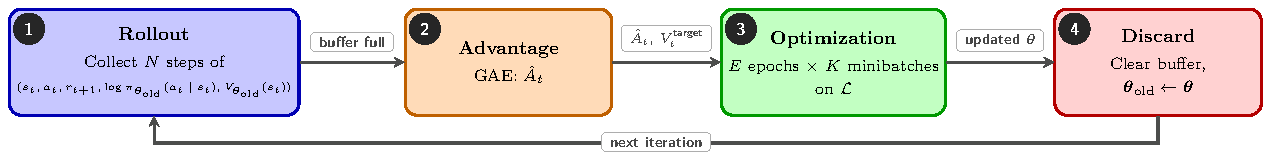
\includegraphics[width=\textwidth]{chapters/03_reinforcement_learning/figures/ppo_cycle.pdf}
    \caption[PPO training cycle]{PPO training cycle: rollout (1), GAE (2), clipped optimization (3), and buffer discard (4).}
    \label{fig:ppo-cycle}
\end{figure}

Figure~\ref{fig:ppo-cycle} illustrates the PPO training cycle, which proceeds in four steps at each iteration.

\paragraph*{Step 1: Rollout Collection.} The agent collects $N$ environment steps with $\pi_{\boldsymbol{\theta}_{\text{old}}}$ and stores them as tuples $(s_t, a_t, r_{t+1}, \log \pi_{\boldsymbol{\theta}_{\text{old}}}(a_t \mid s_t), V_{\boldsymbol{\theta}_{\text{old}}}(s_t))$ in a buffer.

\paragraph*{Step 2: Advantage Computation.} GAE walks backward through the buffer to compute a fixed advantage $\hat{A}_t$ for each step (Equation~\ref{eq:gae}).

\paragraph*{Step 3: Optimization.} The buffer is shuffled into $K$ minibatches and reused for $E$ epochs. At each minibatch, the network recomputes the new $\pi_{\boldsymbol{\theta}}(a_t \mid s_t)$ against the stored $\pi_{\boldsymbol{\theta}_{\text{old}}}$ to form $\rho_t$, then takes a gradient step on $\mathcal{L}$ (Equation~\ref{eq:ppo-loss}). As $\boldsymbol{\theta}$ evolves across these $K{\times}E$ updates, $\rho_t$ drifts from $1$; the clipping bounds this drift and prevents the policy from straying too far from the collected data, allowing multiple passes while remaining approximately on-policy.

\paragraph*{Step 4: Cycle Restart.} The buffer is discarded and $\boldsymbol{\theta}_{\text{old}} \leftarrow \boldsymbol{\theta}$ before restarting the cycle.

\subsection{PPO for MicroRTS}
\label{sec:ppo-microrts}

\begin{figure}[!ht]
    \centering
    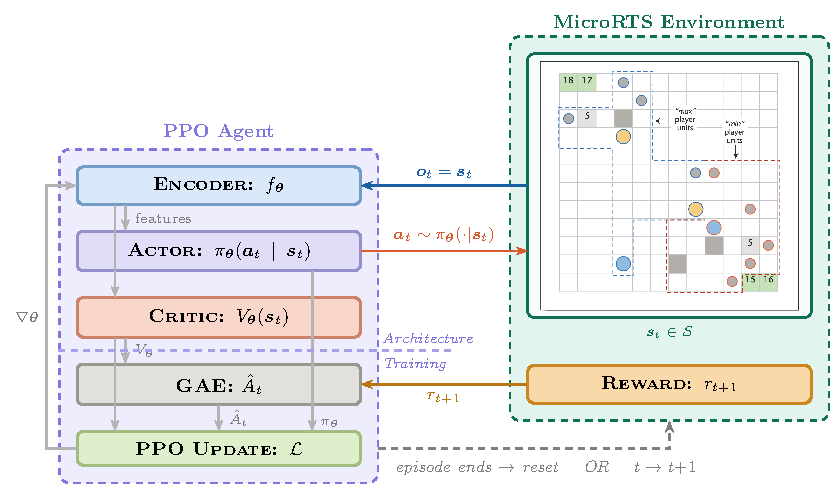
\includegraphics[width=\textwidth]{chapters/03_reinforcement_learning/figures/ppo_loop.pdf}
    \caption[PPO training loop applied to MicroRTS]{PPO training loop applied to MicroRTS. At each timestep, the agent receives an observation and produces an action; the environment returns a reward and advances the game state.}
    \label{fig:microrts-ppo-loop}
\end{figure}

Figure~\ref{fig:microrts-ppo-loop} shows the PPO loop instantiated for MicroRTS. The shared encoder $f_{\boldsymbol{\theta}}$ processes the game state $\boldsymbol{s}_t$ and feeds both the actor and critic. The actor samples an action $\boldsymbol{a}_t$, which is applied to the environment to produce the next state $\boldsymbol{s}_{t+1}$ and reward $r_{t+1}$. GAE combines the critic's estimate $V_{\boldsymbol{\theta}}$ with the reward to compute advantages $\hat{A}_t$, which drive the PPO update of the shared parameters $\boldsymbol{\theta}$ via the objective $\mathcal{L}$. The concrete design choices fill the remainder of this thesis: observation encoding, action representation, and reward signals are covered in Chapter~\ref{chap:python_bridge}; neural network architectures in Chapter~\ref{chap:architectures}; and training enhancements in Chapter~\ref{chap:training-system}.